\chapter{Plataforma de desarrollo}
\label{cap:capitulo3}

\begin{flushright}
\begin{minipage}[]{10cm}
\emph{Cualquier cosa que pueda ser automatizada, será automatizada..}\\
\end{minipage}\\

Robert Cannon, \textit{Título}\\
\end{flushright}

\vspace{1cm}

En este capítulo se detallan los recursos hardware y software empleados para llevar a cabo el desarrollo de la aplicación. A nivel hardware, se han utilizado dos maquetas didácticas de automatización industrial, cada una equipada con un PLC, junto con una interfaz HMI y un brazo robótico colaborativo de la empresa Universal Robots (UR). En cuanto al software, se han utilizado distintos entornos de desarrollo específicos para cada dispositivo: el software TIA Portal para la programación de los PLCs y la configuración de la HMI, y la plataforma URSim para la simulación y control del brazo robótico. Además, se han empleado librerías propias de los fabricantes, sistemas operativos compatibles con las herramientas utilizadas y conexiones mediante protocolos estándar de comunicación industrial como Profinet. Aparte de la programación individual de cada componente del sistema, se ha llevado a cabo el montaje completo y el conexionado de todos los elementos desde su estado inicial de fábrica.

\section{Estación distribución}

La estación de distribución con cinta transportadora de Festo Didactic es un módulo del sistema MPS (Modular Production System) que simula una parte de una línea de producción automatizada. Su función principal es clasificar, alinear y transportar piezas de trabajo desde un punto de alimentación hacia otras estaciones del sistema \cite{estacion_distribucion}. Este sistema está diseñado para la formación técnica en automatización industrial, permitiendo a estudiantes y profesionales aprender a manejar sensores, actuadores, sistemas neumáticos, cintas transportadoras y PLCs. En la tabla \ref{fig:estacion_distribucion_3} se detallan las características generales del sistema: \\

\begin{figure} [h!]
  \begin{center}
    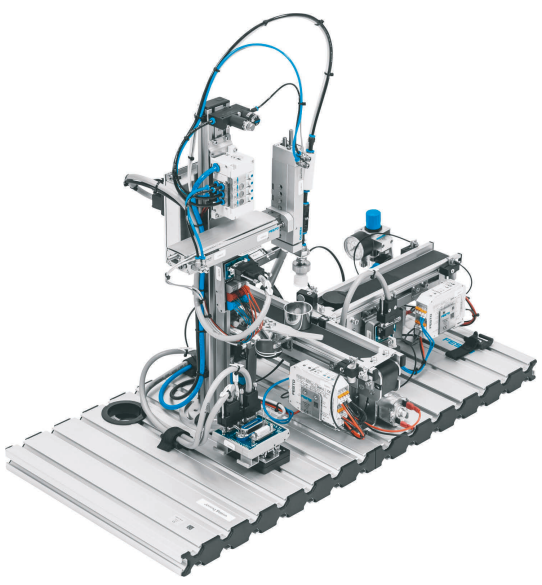
\includegraphics[width=11.5cm]{figs/estacion_distribucion_1}
  \end{center}
  \caption{\centering Estación distribución. \cite{estacion_distribucion}}
  \label{fig:estacion_distribucion_1}
\end{figure} 

\begin{figure} [h!]
  \begin{center}
    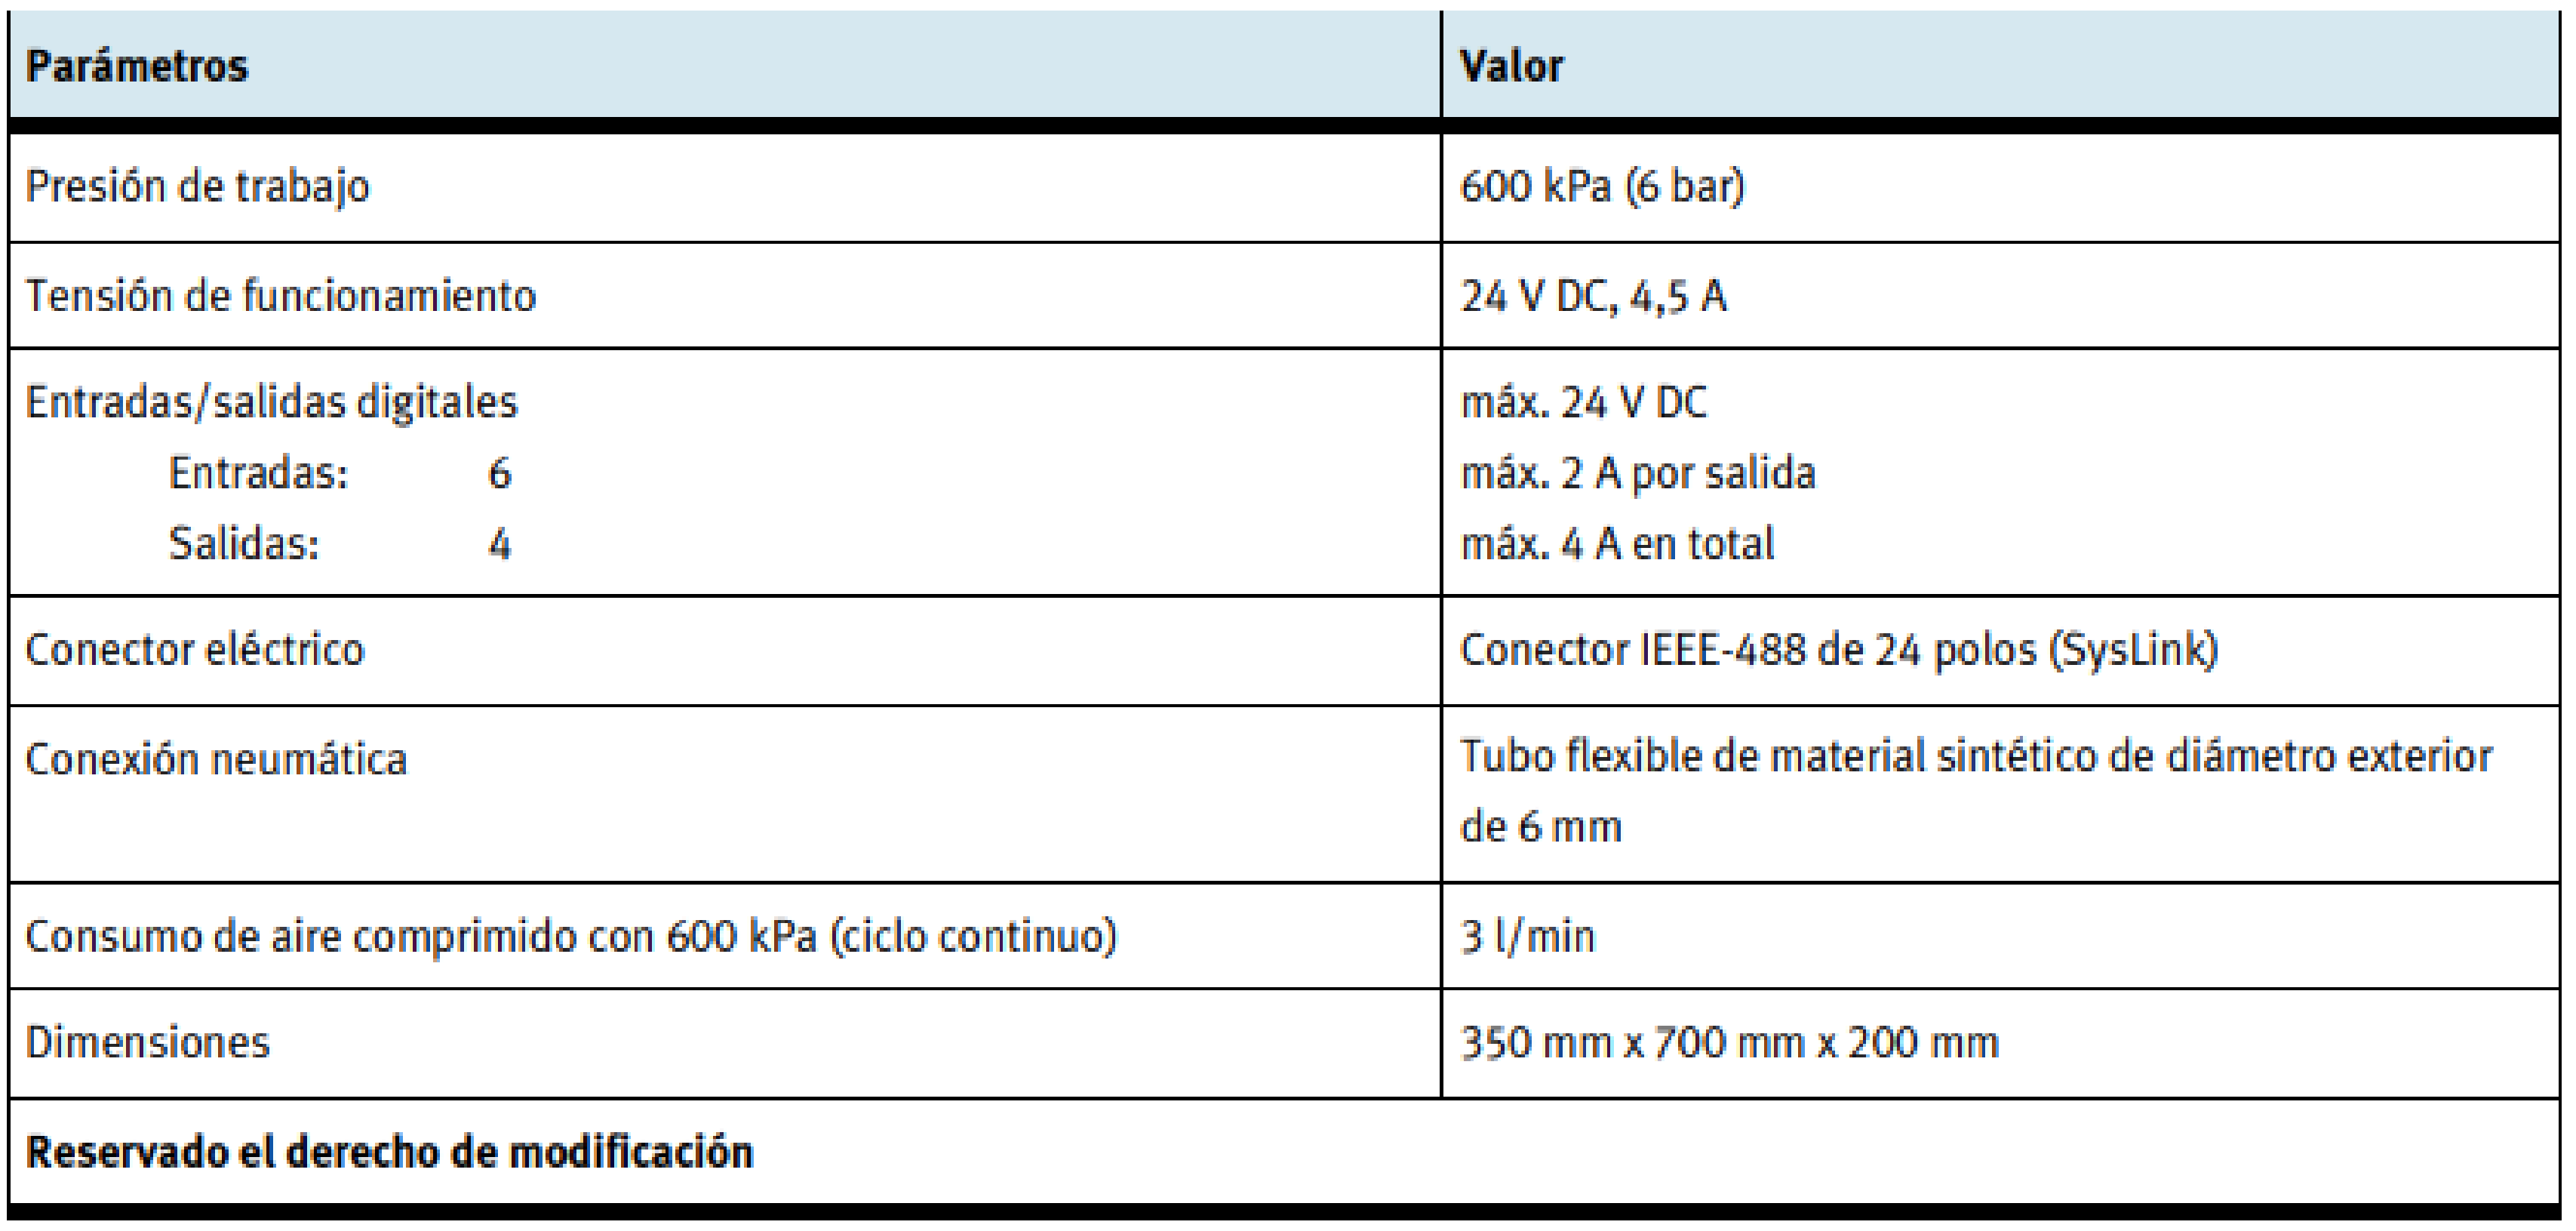
\includegraphics[width=15cm]{figs/estacion_distribucion_3}
  \end{center}
  \caption{\centering Características generales de la etación distribución. \cite{estacion_distribucion}}
  \label{fig:estacion_distribucion_3}
\end{figure} 

\clearpage

Las piezas utilizadas en las estaciones MPS de Festo Didactic suelen estar diseñadas en tres colores: rosa, negro y aluminio. Estas piezas representan distintos tipos de materiales o componentes y las diferencias de color permiten que los sensores ópticos las distingan fácilmente, lo que facilita su clasificación, inspección o tratamiento diferenciado por el sistema automatizado. Cada pieza mantiene dimensiones normalizadas para un manejo preciso y repetible y vienen equipadas con una tapa la cual puede ser colocada en estas para ofrecer mayor libertad al crear el proceso automático \\

La estación distribución está formada por los siguientes componentes:

\begin{itemize}
   \item \textbf{Stapelmagazin (almacén de piezas):} Sistema de alimentación que permite introducir piezas de trabajo de manera ordenada a mitad de la cinta transportadora. Funciona como un cargador vertical donde las piezas se apilan y se liberan una a una mediante un actuador neumático (máximo 7 piezas) \cite{estacion_distribucion}. Está diseñado para asegurar una alimentación controlada y repetible en los procesos de automatización \cite{estacion_distribucion}.
   
    \item \textbf{Cinta transportadora:} Encargada de desplazar las piezas entre las estaciones. Puede moverse en ambas direcciones. 
    
     \item \textbf{Separador:} Actuador neumático situada al inicio de la cinta cuya función es controlar el flujo de piezas en la cinta transportadora. Si se activa retiene las piezas provenientes del inicio de la cinta y da paso a las almacenadas en el almacén de piezas \cite{estacion_distribucion}.
     
      \item \textbf{Sensor para la distinción de piezas:} El sistema viene equipado con un módulo extra situado a la mitad de la cinta el cual es capaz de distinguir el color de la pieza. Si la pieza es de color negro se activa un bit, si es rosa se activan dos y si es metálica tres \cite{estacion_distribucion}.

    \item \textbf{Sensores:} La estación posee sensores ópticos y de proximidad que detectan la presencia, posición o características de las piezas, proporcionando datos al PLC.

    \item \textbf{Estructura mecánica modular:} Bastidor de perfiles de aluminio que soporta todos los componentes y permite su integración con otras estaciones del sistema MPS \cite{estacion_distribucion}.
\end{itemize}

\clearpage

\begin{figure} [h!]
  \begin{center}
    \includegraphics[width=17cm]{figs/estacion_distribucion_2}
  \end{center}
  \caption{\centering Componentes de la estación distribución.}
  \label{fig:estacion_distribucion_2}
\end{figure} 

\section{Estación unión}

La estación de unión de Festo Didactic simula un proceso industrial en el que se unen dos piezas mediante un actuador neumático equipado con una ventosa (Pick\&Place) \cite{estacion_union}. El objetivo de esta estación es colocerle o retirerle las tapas a las piezas que estén correctamente orientadas y así terminar la secuencia. La estación está compuesta por un brazo neumático, dos cintas para mover las piezas y tapas, sensores que detectan su presencia y adicionalmente un sensor cuya función es detectar la orientación de las piezas \cite{estacion_union}. Esta estación permite realizar prácticas de automatización como control secuencial, posicionamiento y verificación del montaje. Es ideal para formación técnica en tareas típicas de ensamblaje automatizadas. Además se adjuntan las características generales de la estación como se puede ver en el gráfico \ref{fig:estacion_union_3}:

\clearpage

\begin{figure} [h!]
  \begin{center}
    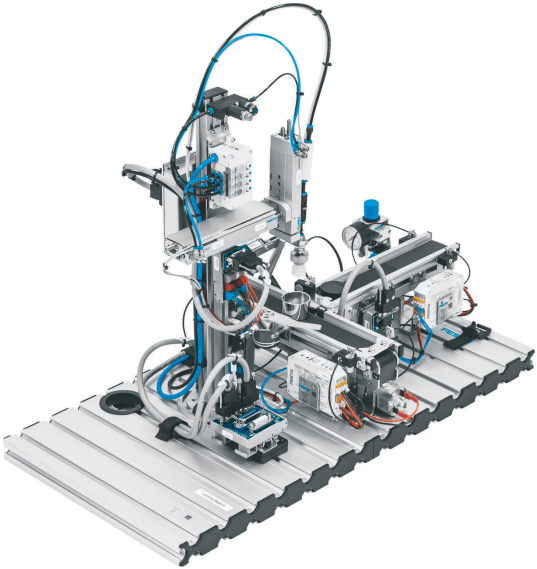
\includegraphics[width=10.75cm]{figs/estacion_union_1}
  \end{center}
  \caption{\centering Estación unión. \cite{estacion_union}}
  \label{fig:estacion_union_1}
\end{figure} 

\begin{figure} [h!]
  \begin{center}
    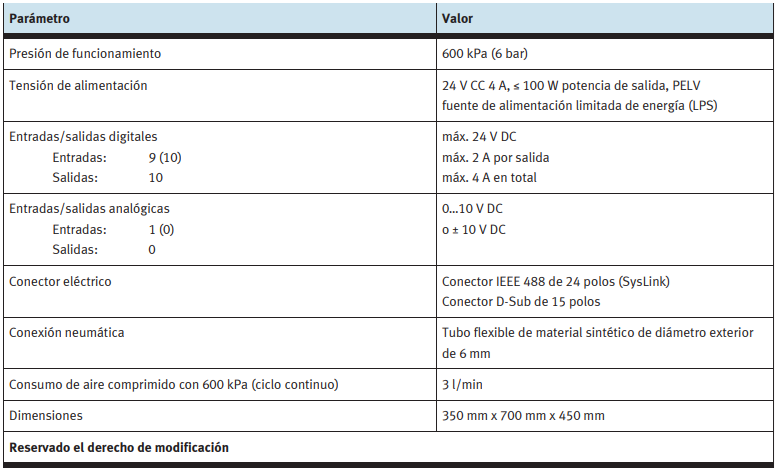
\includegraphics[width=15cm]{figs/estacion_union_3}
  \end{center}
  \caption{\centering Características generales de la estación unión. \cite{estacion_union}}
  \label{fig:estacion_union_3}
\end{figure} 

El Módulo de \textbf{Cinta Transportadora 1} transporta, separa y acumula piezas de hasta 40 mm de diámetro. Está impulsado por un motor de corriente continua con control de velocidad y dirección, y utiliza sensores ópticos para detectar la presencia de piezas al inicio, medio y al final de la cinta \cite{estacion_union}. Un electroimán que actúa como retenedor permite detener y liberar piezas individualmente a la altura del brazo, y un sensor difuso con salida digital y analógica identifica la orientación de las piezas el cual se ayuda de un retenedor para poder hacerlo correctamente sin que se mueva la pieza \cite{estacion_union}.

El Módulo de \textbf{Cinta Transportadora 2} tiene funciones similares, pero está diseñado para manejar tanto cuerpos de piezas como tapas. También utiliza un motor de corriente continua y sensores ópticos para controlar el flujo de materiales \cite{estacion_union}.

El Módulo \textbf{Pick\&Place} es un manipulador de dos ejes que utiliza carros deslizantes de precisión y sensores de proximidad para detectar las posiciones finales. Puede equiparse con una ventosa de fuelle o un gripper paralelo para agarrar las piezas, y cuenta con un filtro de vacío y un presostato para asegurar una sujeción fiable \cite{estacion_union}. La fuerza del eje vertical puede ajustarse mediante un regulador de presión, y el módulo incluye todos los componentes necesarios para su funcionamiento, como generador de vacío, válvulas y conexiones eléctricas \cite{estacion_union}.

\begin{figure} [h!]
  \begin{center}
    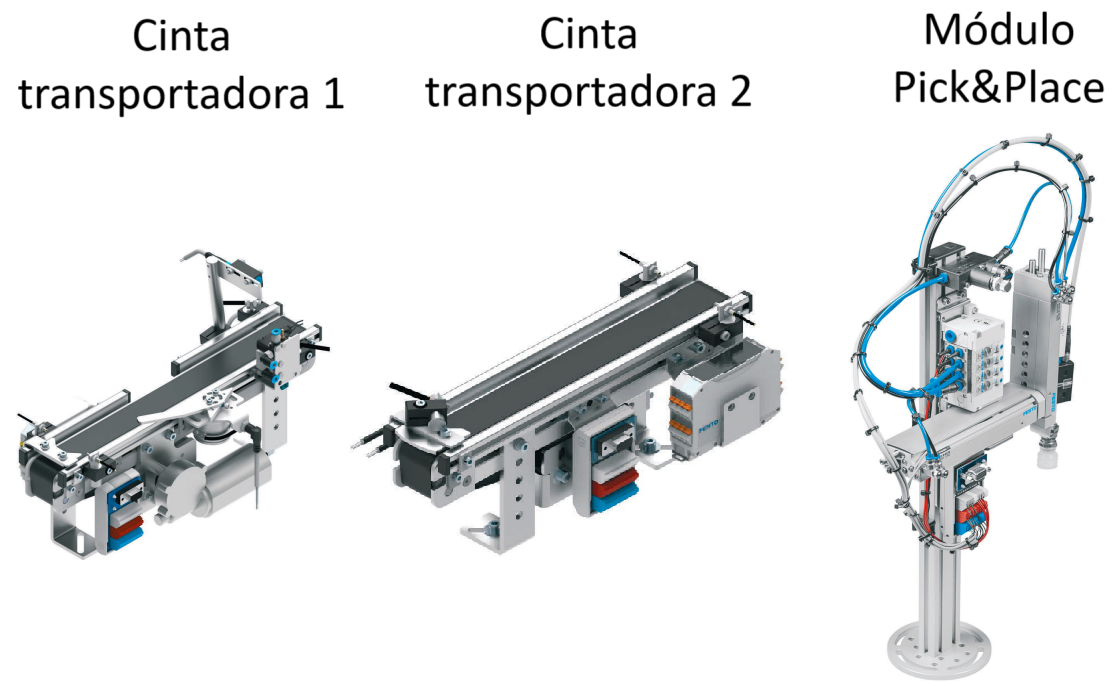
\includegraphics[width=14.5cm]{figs/estacion_union_2}
  \end{center}
  \caption{\centering Componentes de la estación unión. \cite{estacion_union}}
  \label{fig:estacion_union_2}
\end{figure} 

\begin{figure} [h!]
  \begin{center}
    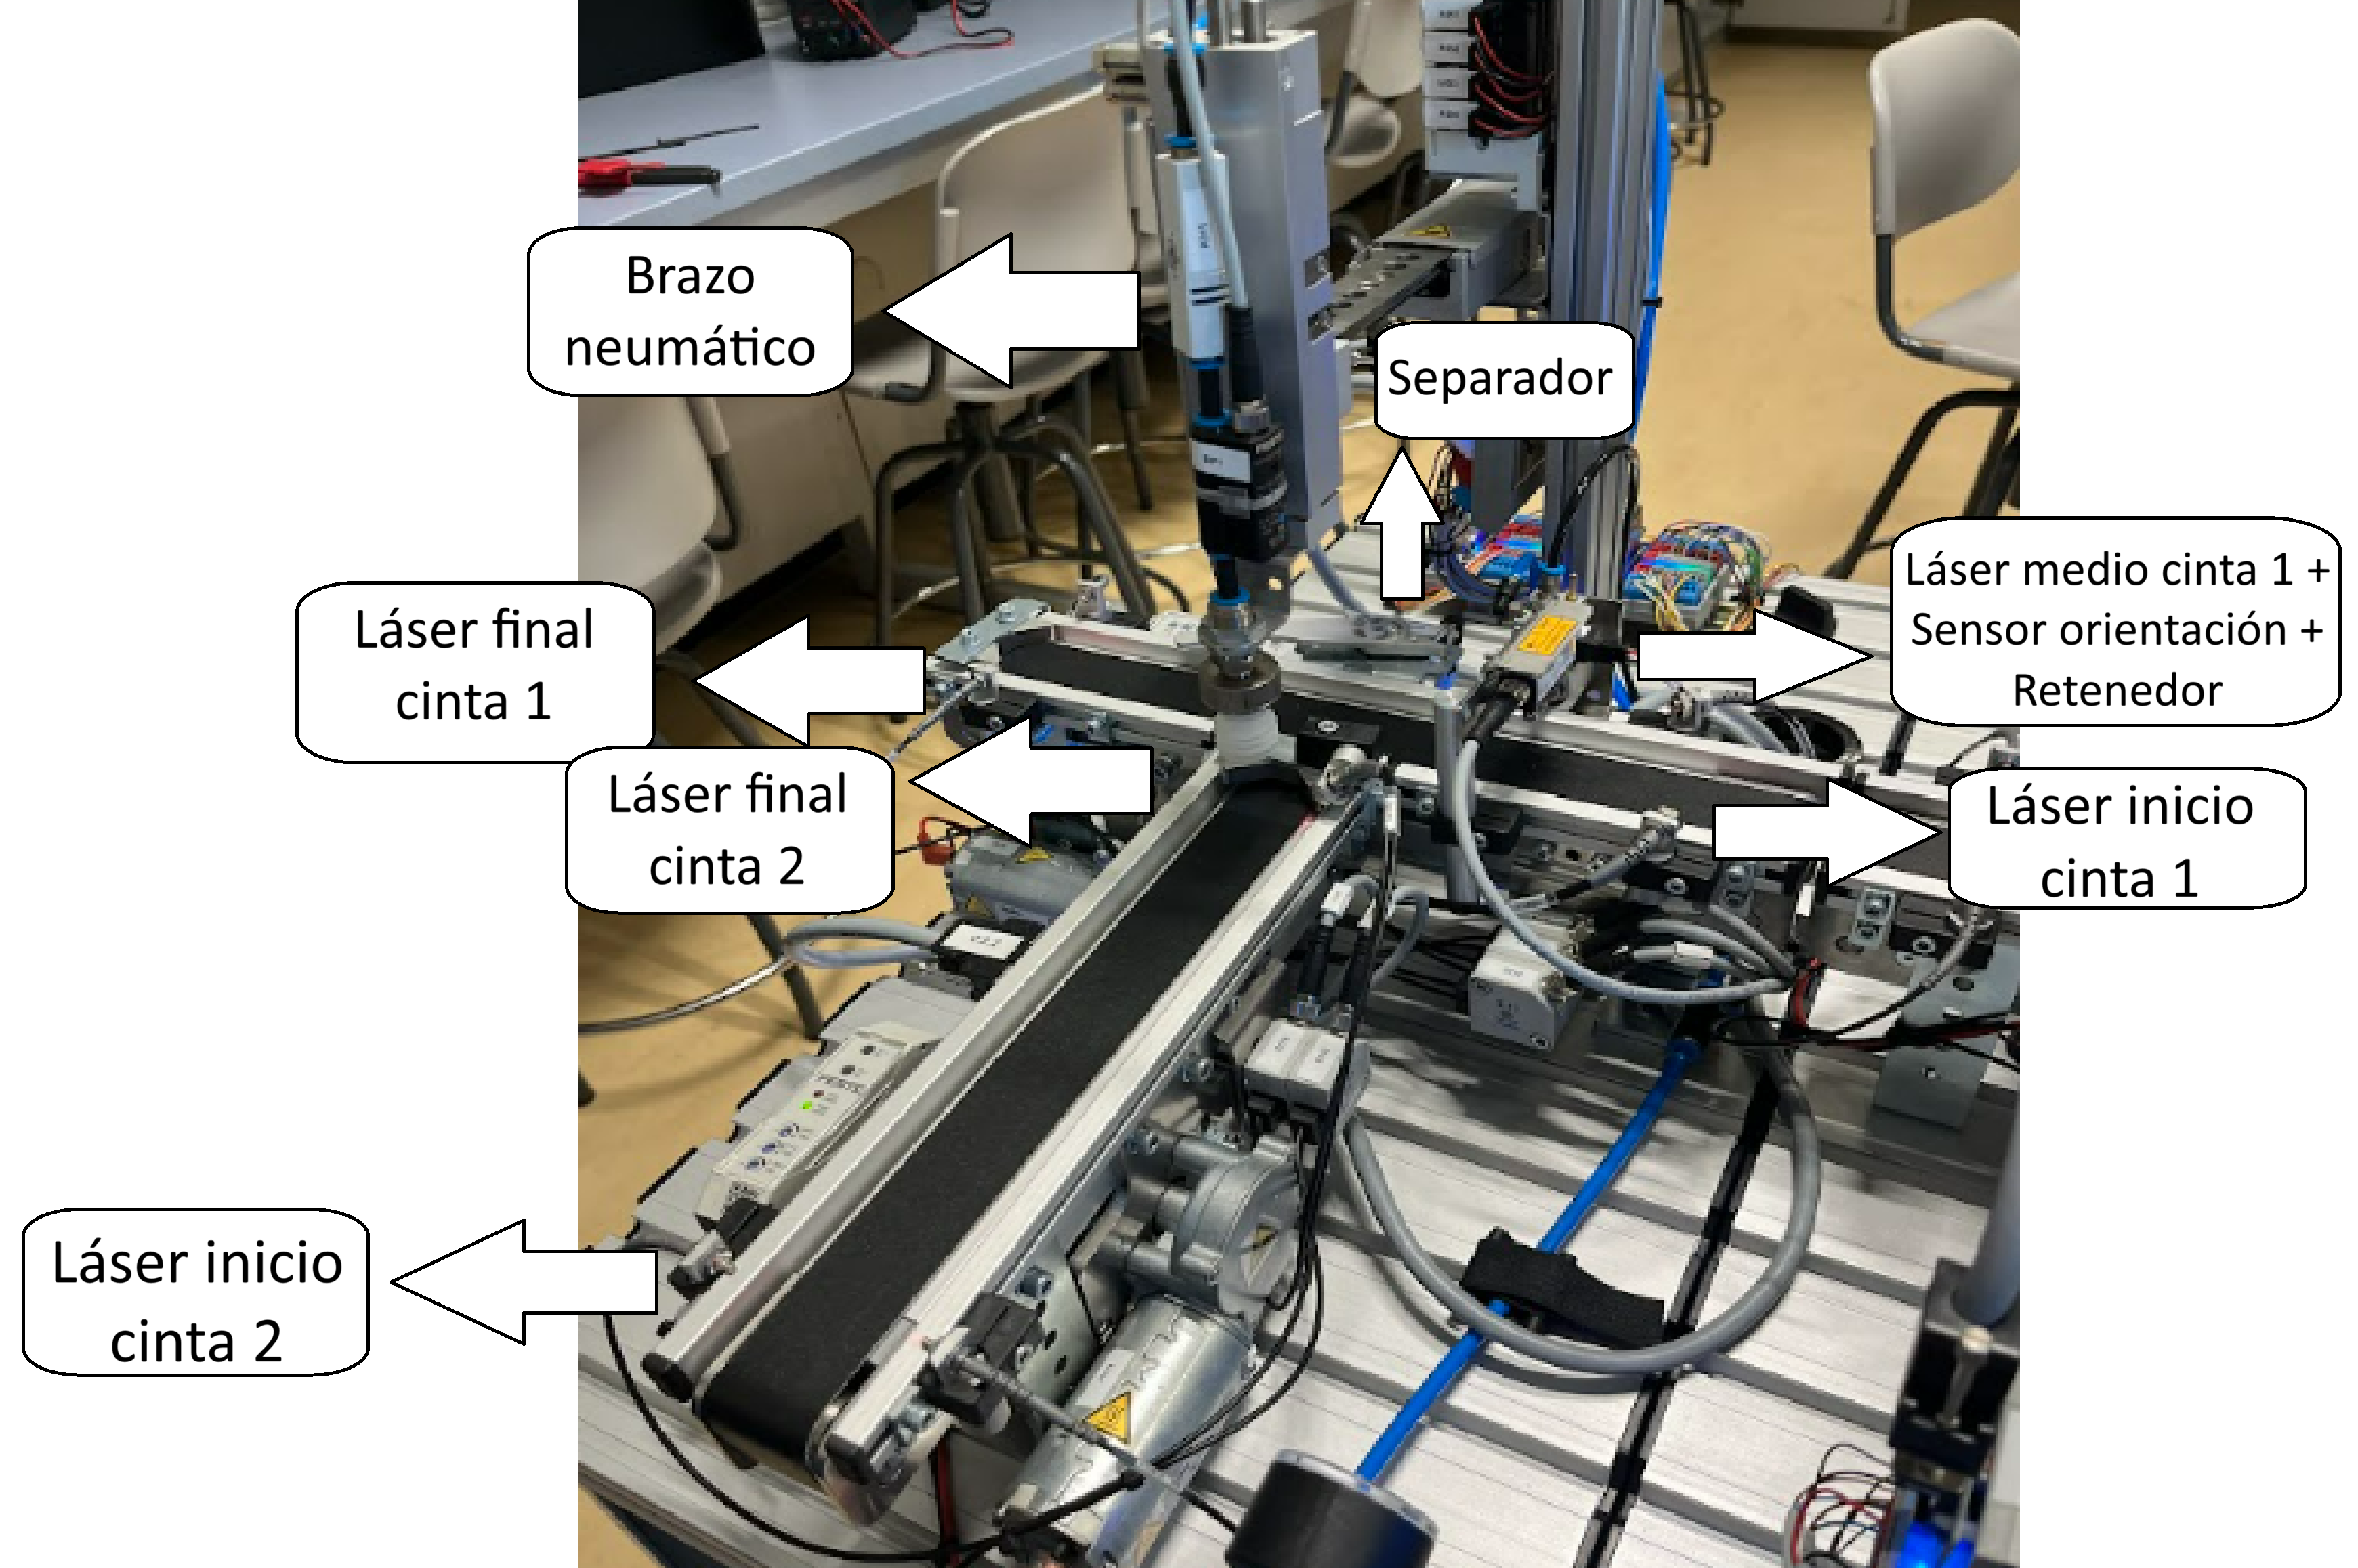
\includegraphics[width=16.5cm]{figs/estacion_union_4}
  \end{center}
  \caption{\centering Componentes de la estación unión.}
  \label{fig:estacion_union_4}
\end{figure} 

\section{PLCs Siemens 1200s}

Para la elaboración de este trabajo se ha utilizado el PLC Siemens S7-1200, concretamente el modelo \textbf{6ES7 215-1BG40-0XB0}. Este modelo forma parte de la familia de controladores compactos de Siemens, ampliamente utilizados en aplicaciones de automatización industrial. El PLC corresponde a la CPU 1215C con alimentación AC/DC y salidas a relé, lo que le otorga una gran versatilidad para controlar y supervisar sistemas de pequeña y mediana escala \cite{PLC_siemens}.

Entre sus características más destacadas se encuentran sus 14 entradas digitales de 24 V DC, 10 salidas digitales tipo relé de 2 A, 2 entradas analógicas (0–10 V DC) y 2 salidas analógicas (0–20 mA DC) \cite{PLC_siemens}. Esta combinación de entradas y salidas permite conectar una gran variedad de sensores y actuadores directamente al PLC sin necesidad de módulos adicionales, lo que reduce costes y espacio en armarios de control.

En términos de comunicación, esta CPU incorpora dos puertos PROFINET con función de switch integrado, lo que facilita su integración en redes industriales y la comunicación con dispositivos HMI, otros PLCs o sistemas SCADA \cite{PLC_siemens}. Además, es compatible con protocolos de comunicación abiertos como TCP/IP, ISO-on-TCP, UDP y MODBUS, y permite el uso de servidor OPC UA mediante licencia, una característica clave para entornos de Industria 4.0 \cite{PLC_siemens}.

\begin{figure} [h!]
  \begin{center}
    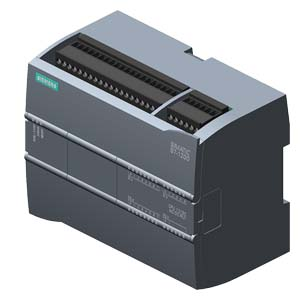
\includegraphics[width=8cm]{figs/PLC_siemens}
  \end{center}
  \caption{\centering PLC Siemens 1215 AC/DC/RLY. \cite{PLC_siemens}}
  \label{fig:PLC_siemens}
\end{figure} 

Su programación se realiza a través del software \textbf{STEP 7 (TIA Portal)} versión V20 o superior, ofreciendo compatibilidad con lenguajes como KOP (diagrama de contactos), FUP (diagrama de funciones) y SCL (lenguaje estructurado) \cite{PLC_siemens}. También dispone de funciones tecnológicas avanzadas como control PID, contadores de alta velocidad (hasta 100 kHz), y posicionamiento, lo cual amplía sus capacidades para aplicaciones más exigentes \cite{PLC_siemens}.

En cuanto a su hardware, presenta una memoria de trabajo de 200 kB y una memoria de carga de 4 MB, además de la posibilidad de insertar una tarjeta SIMATIC Memory Card para ampliar almacenamiento o realizar copias de seguridad \cite{PLC_siemens}. El diseño compacto (130 × 100 × 75 mm) y el grado de protección IP20 lo hacen ideal para entornos industriales controlados.

\section{HMI}

\section{Brazo UR5}





